%!TEX root=../Vorlage_DA.tex
%	########################################################
% 				Darstellung der Variablen
%	########################################################
\chapter{Darstellung der Variablen}

Die Darstellung der Variablen während der Laufzeit ist eine essentielle Funktion der Benutzeroberfläche. Die anschauliche und übersichtliche Darstellung soll dem Benutzer ein fundiertes Verständnis für den Ablauf des Programmes und die Rolle der Variablen sowie deren Gültigkeitsbereiche vermitteln.

%	--------------------------------------------------------
% 	Unterschiede zu einem Debugger
%	--------------------------------------------------------
\section{Unterschiede zu einem herkömmlichen Debugger}
Die Idee der Variablendarstellung während der Laufzeit gleicht einem Debugger. Der Begriff Debugmodus kommt besonders im Sourcecode, aber auch in der Dokumentation und in der Benutzeroberfläche immer wieder vor. Allerdings unterscheidet sich die Darstellung von Programmabläufen und Variablen in C Compact in einigen Punkten von herkömmlichen Debuggern:
\begin{itemize}
\item Während die Debugger professioneller Entwicklungsumgebungen eine Hilfestellung für erfahrene Programmierer sind, ist der Debugmodus von C Compact besonders auf Anfänger ausgerichtet.
\item Die Darstellung der Variablen ist übersichtlich und fester Bestandteil der Beutzeroberfläche von C Compact. Einsteiger und unerfahrene Programmierer sollen von Anfang an mit dem Debugger in Berührung kommen.
\end{itemize}

%	--------------------------------------------------------
% 	Einführung + Erklärung Variablendarstellung
%	--------------------------------------------------------
\section{Darstellungsform der Variablen}

Zur Darstellung wurden zwei Konzepte verfolgt:
\begin{enumerate}
\item Die Darstellung des Call Stacks als Liste mit separaten Tabellen für die lobalen und lokalen Variablen
\item Die Darstellung aller Variablen als Baum, wobei lokale Variablen Funktionen untergeordnet sind und sich globale Variablen auf derselben Ebene wie Funktionen befinden
\end{enumerate}

In den ersten Versionen der Benutzeroberfläche wurden die Variablen wie in Punkt 1 beschrieben dargestellt. Bereits während unseres Praktikums am Institut für Systemsoftware der JKU wurde die zweite Form der Variablendarstellung theoretisch entworfen. Die erste vollständige Implementierung erfolgete noch während den Sommerferien.
\newline

In der ersten numerierten Version (Alpha 1.0) waren noch beide Darstellungsformen vorhanden und konnten vom Benutzer ausgewählt und gewechselt werden. Allerdings waren diese beiden Darstellungsformen sehr unterschiedlich implementiert, was anfangs dazu führte, dass die Darstellung der Variablen als Baum nicht mehr als ein zusätzliches Feature ohne den vollen Funktionsumfang der Variablendarstellung als Call Stack war.
\newline

Für die Version Alpha 1.1 sollte ursprünglich das Variablendarstellungssystem so verändert werden, dass beide Anzeigemodi über ein gemeinsames Interface angesprochen werden können. Nach ausführlicher Besprechung und Evaluierung der unterschiedlichen Variablendarstellungen haben wir aber beschlossen, die Variablen nur als Baum darzustellen. Dadurch haben sich folgende Vorteile ergeben:
\begin{enumerate}
\item Die implementierung einer neuen Funktion bei der Variablenanzeige muss nur noch einmal erfolgen und nicht für jeden Anzeigemodus extra vorgenommen werden.
\item Daraus resultiert auch ein durchdachteres und einfacheres Bedienungskonzept der Benutezroberfläche, da dieses nur an eine Variablendarstellung angepasst werden muss.
\item Davon profitiert zuletzt der Benutzer, der eine komplette und sauber implementierte Darstellung und Erklärung für die Variablen während des Programmablaufes vorfindet.
\end{enumerate}

%	--------------------------------------------------------
% 	Darstellung in getrennten Tabellen
%	--------------------------------------------------------
\section{Darstellung der Variablen in getrennten Tabellen}

Diese Form der Variablendarstellung wurde erstmals im Dokument Ausführungsumgebung für C-- von Herrn Professor Blachek beschrieben und nach dieser Vorlage implementiert.
\begin{figure}
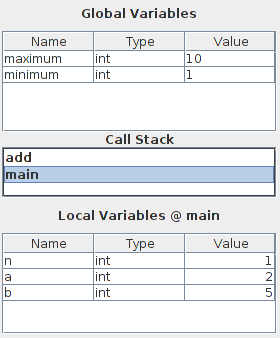
\includegraphics[width=4cm]{./media/images/gui/var/callstack.png}
\caption{Darstellung der Variablen in separaten Tabellen}
\label{var_sep}
\end{figure}

%	--------------------------------------------------------
% 	Darstellung als Baum
%	--------------------------------------------------------
\section{Darstellung der Variablen als Baum}

Die Darstellung der Variablen in Form einer Baumstruktur hat den Vorteil, dass alle Variablen in einem Feld untergrbracht sind und der heriarchische Zusammenhang sofort ersichtlich ist.

Dieser Darstellungsmodus ist als TreeTable, eine Kombination aus JTree und JTable, implementiert.
